\documentclass{standalone}

\usepackage{tikz}    

\begin{document}
		
	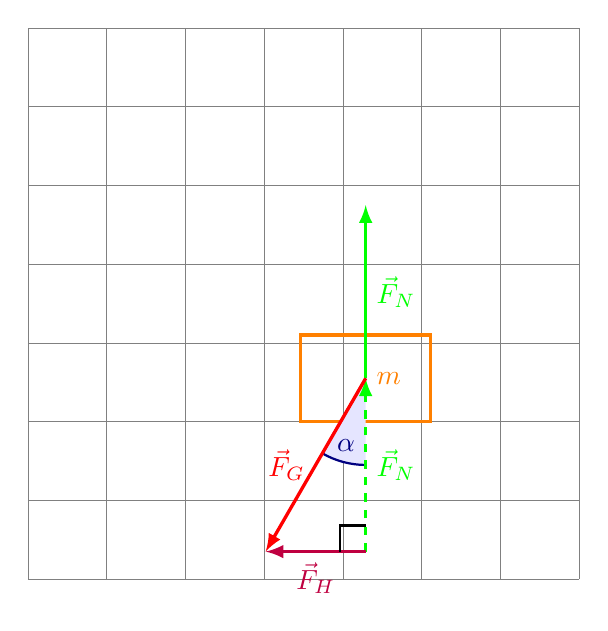
\begin{tikzpicture}
		
		
		%Raster im Hintergrund
		\draw[step=1, gray, very thin] (0,0) grid (7,7);
		%Grundlinie		
		
		%Winkel
		%\filldraw[fill=blue!10, draw=blue!50!black, thick] (0,0) -- (2,0) arc(0:30:2);
			%{$\color{green!50!black}\alpha$};
		%Gerade nach rechts 	
		%\draw [thick] (0,0) -- (10,0);
		
		%Schiefe Ebene 
		%\draw [thick] (0,0) -- (9,5.196);
		
		%\draw (3,0) arc(0:20:3);
		
		\begin{scope}[xshift=3.464cm, yshift=2cm, rotate=0, scale=1.1]

			\coordinate (A) at (0.75,0.5);
			\coordinate (B) at (0.75,-1.5);
			
    		\draw [orange, very thick] (0,0) rectangle (1.5,1) node [midway, right] {$m$} {} ;
    		\begin{scope}[xshift=0cm, yshift=0, rotate=0, scale=1]
    			\begin{scope}[xshift=0.75cm, yshift=0.5cm, rotate=-120, scale=1]
    				\filldraw[fill=blue!10, draw=blue!50!black, thick] (0,0) -- (1,0) arc(0:30:1) node [midway, above, xshift=1pt, yshift=0, blue!50!black] {$\alpha$} {};
    			\end{scope}
    			%\draw [orange] (0,0) -- (1.5,1);
    			%\draw [orange] (0,1) -- (1.5,0);
    			\draw [-latex, very thick, dashed, green] (B) -- (A) node [midway, right] {$\vec{F}_N$} {};
				\draw [-latex, very thick, green] (A) -- ++(0,2) node [midway, right] {$\vec{F}_N$} {};
    			\draw [-latex, very thick, purple] (B) -- ++(-1.1547,0) node [midway, below] {$\vec{F}_H$} {};
    			\draw [-latex, very thick, red] (A) -- ++(-1.1547,-2) node [midway, left] {$\vec{F}_G$} {};
    			\draw [thick](0.45,-1.5) -- (0.45,-1.2) -- (0.75,-1.2);  
    		\end{scope}		    		
  		\end{scope}
		
	\end{tikzpicture}
\end{document}